\documentclass[]{article}

%opening
\title{%
	EDB: A Debugger for Ethereum's Programming Languages \\
	\bigskip	
	\bigskip									
	\large	Proposal for Computer Projects 2018 \\
	\large University of Scranton}

\author{Andrew Plaza}
\usepackage{graphicx}
\usepackage[font=small,labelfont=bf]{caption}
\begin{document}

\maketitle
\newpage
\tableofcontents
\newpage

\section{Context}
\subsection{Blockchain: What Is It?}

In recent years, blockchain and digital currencies have rocketed in popularity. Many have realized blockchain technology has the potential to revolutionize society. For instance, IBM has recently released a tracker for supply-chains built upon the blockchain.\footnote{IBM \textit{Blockchain for Supply Chain} https://www.ibm.com/blockchain/supply-chain/} In general, blockchain currencies can be thought of as a decentralized monetary system shared across the world via the internet, while remaining almost free to use. One may compare the basic functions of a cryptocurrency to the functions of a bank. Apart from how one uses it, owning a variety of cryptocurrency is no different than owning some amount of U.S dollars. For instance, owning one 'Bitcoin' has an equivalent value in USD (currently, 1 Bitcoin is equal to 8513.08\$). Despite being unofficial and not currently endorsed by any government, value is attributed to these currencies through adoption and speculative investment. Much like stocks, the value of these currencies is very volatile, so many have found it to their advantage to speculate on the price in the hopes of earning some money.

Cryptocurrency, however, does not strive to copy and replace the traditional banking system. For example, unlike U.S currency, no one can just 'print' more Bitcoin. Rather, Bitcoin has a cap of 21 million coins. No more Bitcon can ever be created once 21 million Bitcoin exist. In this respect, cryptocurrencies are more like gold than normal USD. Despite this, cryptocurrencies put forth clear advantages to traditional banking. They are decentralized and cryptographically secure. Unlike traditional banking, no 'middleman' exists or is necessary to make transactions with bitcoin. Furthermore, transactions are validated and confirmed through a network of 'miners'. All this works because of blockchain which is by its very definition and use-case decentralized. The blockchain solves one of the most prominent roadblocks with a digital and decentralized money system, which can be explained through the 'double-spend' problem. The double-spend problem occurs when some person (person A) owns some amount of money, and tries to spend more money than they actually own. For example, person A owns 50\$. Person A sends some other individual 50\$. At the same time, Person A creates the same exact transaction but to yet another individual. Clearly, both these transactions cannot go through, since Person A only owns 50\$, not 100\$. Blockchain solves this issue.

In essence, blockchain is a ledger that can be downloaded by anyone with an internet connection. This blockchain serves as 'memory' for digital monetary systems. Anyone who downloads and uses a blockchain on their computer can be said to be a 'blockchain node'. Anytime a transaction is created, it is recorded onto the blockchain (the ledger), which then updates, via the internet, every other blockchain anyone else has downloaded. This blockchain keeps track of every single transaction ever made, therefore keeping track of how much money everybody owns.  Before a transaction is recorded onto the blockchain, however, it must be confirmed and validated. This is where a network of miners come in, and a process of validation known as 'proof of work' occurs. A 'miner' in this context is simply a individual who has designated to contribute some processing power for the good of the blockchain network. Proof-of-work, then, is the process a few miners (chosen at random) undertake by running blockchain nodes. Upon receiving a new transaction, the miners run through every past transaction a user made in order to make certain money exists and can be transfered. In order to remain decentralized, more than one miner is chosen, and they must all agree to the validity of a transaction. Since these miners are connected over the internet, agreeing becomes a simple matter of first individually checking the validity of a transaction, and then checking if the other miners also consider the transaction valid. If a transaction cannot be confirmed, that is not all miners agree on its validity, it is considered invalid, and so the blockchain is not updated with this transaction. A simple and useful way to conceptualize the blockchain is as a linked-list of transactions that everyone owns, and is updated if a transaction is found to be valid.
 
The process of confirmation and validation that miners undertake, however, must be executed by a computer processor (in many cases, multiple computer processors) somewhere in the world. This means someone's computer needs energy (which costs money) for the computing power required to verify a transaction. Since very few people would offer up their resources to process arbitrary transactions for free, there must be some incentive involved for users to offer up their processing power. For cryptocurrencies, the incentive becomes generating more of the cryptocurrency one is mining for. At a basic level, however, adding some transaction to a blockchain is a simple activity and not at all resource-intense. It would be very easy to add many of one currency to a blockchain if there was nothing to stop it, therefore drastically increasing supply and making the currency worthless. In order to solve this, mining new transactions or 'adding a new block', is intentionally designed to be very resource-intensive through the use of some very difficult mathematical problems. There is a prescribed difficulty for these math problems that goes up over time. In addition, the amount of currency generated by successfully solving the mathematical problem decreases over time. This makes it impossible to ever reach the ultimate supply cap of a currency. 

The blockchain is also cryptographically secure. Blockchain nodes are differentiated through private-public key encryption. Once a user downloads the blockchain, it encrypts itself and the user receives a private and public key. The public key can be shared with anybody and serves as an address people may send currency to. In the blockchain, transactions made by any one user are associated with this public key. That is, the public key serves as an identifier in the blockchain entry. This doubles as an identification mechanism, too. Before sending a transaction a user must confirm who they are by signing the transaction with their public key, which may only be done if they also own the private key. It becomes very important to keep the private key safe; losing or giving away one's private key leads to the compromise of any and all funds of cryptocurrency owned by that key. 

It becomes useful to think of the blockchain in terms of an infinite state-machine. That is, the machine has a start state but no defined end-state. One may think of each transaction as a state of this machine. A new transaction creates a new unique state for the machine. These states are kept track of by an internal data structure (IE: the linked-list). All of this creates what we know as the blockchain.

Ethereum takes the traditional concept Bitcoin created a step further; Ethereum, another blockchain currency, essentially allows any developer the ability to create their own software on top of Ethereum.\footnote{Gavin Wood, \textit{Ethereum Whitepaper} http://gavwood.com/Paper.pdf} Developers may create their own new state-machines on the Ethereum blockchain, consisting of any state they may want. This new state is also executed by the miners, in addition to updating transactions and completing the mathematical problems required. Since this state is executed by normal computer processors, it has the ability to execute code.

\bigskip
\begin{minipage}{0.9\linewidth}
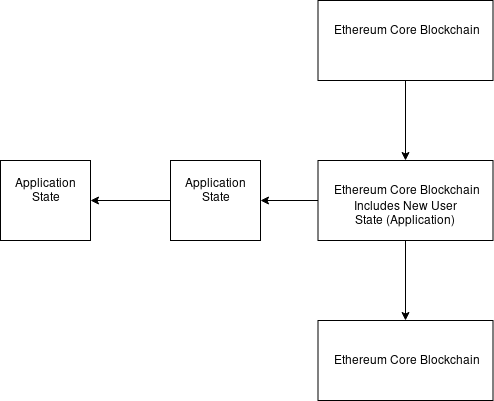
\includegraphics[width=\linewidth]{ethereum-state.png}
\captionof{figure}{A conceptual interpretation of Ethereum's blockchain paired with an application created by a user}
\end{minipage}%
\hfill
\bigskip

Although it would be theoretically possible to create any kind of application imaginable and commit it to the blockchain, in practice it would not be very practical. Because of the way blockchain works, the more resource-intensive a program is, the longer it will take to execute by the miners. Since this, too, takes computational power, the miners need some kind of compensation. In addition, and according to Alan Turing's halting problem, an algorithm to solve whether a program will finish running does not exist.\footnote{Turing, Alan \textit{On Computable Numbers} https://www.cs.virginia.edu/~robins/Turing\_Paper\_1936.pdf} This introduces many problems for Ethereum's blockchain. For example, it would be very easy for a malicious third-party to create and commit a forever-loop to the blockchain and severely limit its functionality. In order to solve this, Ethereum's developers implemented a feature known as 'gas'. Gas is simply Ethereum currency, but in much smaller increments ($1 gas = 2 * 10^{-6}ETH$). Every time an instruction of an application is executed by some processor, it costs a set amount of gas. When a user wants to execute part of an application, a maximum gas-price is set by the user. If the gas price is exceeded during the transactions execution, then the transaction is failed and not validated by Ethereum's network. Gas spent on executing transactions is sent to the miners responsible for running them. Because of gas, the more complex a program becomes, the more expensive it becomes to run. Therefore, a very complex application uploaded to the blockchain may be too expensive for any user to run.

In order to facilitate the developers ability to write software for Ethereum, a set of specialized programming languages were built. These are LLL (Low-Level Lisp-like Language), Solidity, Serpent, and Vyper. These programming languages compile to bytecode, which is processed by the Ethereum Virtual Machine (EVM). The EVM lives within the Ethereum blockchain node downloaded by any user, and is used whenever a user designates themselves as a miner.


\subsection{Who Needs It?}

The Ethereum Open Source community, which includes hobbyist and early-adopter developers, need an intuitive and familiar way of testing their applications written for Ethereum. A debugger with a familiar interface and an emphasis on ease of use, extensibility, and maintainability needs to be developed.

The core of this project concerns the debug API. This API serves as the engine that enables debuggers to be built. In essence, the API will be a process that exposes debug functionality via an inter-process communication (IPC) protocol. Documentation of the IPC protocol allows the development of other debuggers by third-parties for various development environments and workflows by revealing how the API works, and what functions may be called through the IPC mechanism. Essentially, this project is being done in order to enable the development of fully-fledged debuggers. For demonstration and testing purposes, however, two simple interfaces will be developed in addition to the API. These are the command-line interface and the Visual Studio Code plugin. These plugins 'complete' the debugger experience, and work by communicating with the process that is the debug API.

\subsection{Reasons For A New System?}
Currently, debuggers for specialized blockchain programming languages remain either non-existent or extremely limited. The most popular current debugger is an online tool known as an Integrated Developer Experience (IDE) and named 'Remix'.\footnote{\textit{Remix} https://remix.ethereum.org/} Although providing some popular functions of debugging, Remix is cumbersome and complicated to use. Despite this lack of debuggers, however, applications written in Ethereum's programming languages greatly benefit from extensive testing and debugging in order to better ensure security and a seamless user experience.


\subsection{Where Will It Be Used?}
 
This new debugger will be used locally on the developer's machine. The debug API, however, may be used in conjunction with many popular IDE plugin frameworks to build a customized debugging interface.

\subsection{Software Requirements}
In order to develop the debug API, a robust and tested EVM implementation is needed.\footnote{\textit{Parity EVM} https://github.com/paritytech/parity/tree/master/ethcore/evm/src} In addition to this, a compiler for these languages is required to be used. During development, I will use vim as an editor, Rust document generation for documentation of the debug API, and native Rust testing constructs for integration and unit testing.

\subsection{Intended Target Demographic}
The demographic which will exert the most use out of this debugger is the Ethereum Open Source community.

\section{Overview}

\subsection{Problem}
The only current debugger for Ethereum's languages in existence, Remix, is too complicated and cumbersome to use. In addition to this, there is no integration with popular developer IDE's such as Visual Studio Code or IntelliJ. As these specialized languages become more and more popular, more advanced debugging techniques will become more important in order to test applications growing in size and complexity. 

\subsection{Objectives}
\begin{itemize}
	\item Create a debug API supporting at least the Solidity language with a robust and clear API that is well-documented
	\item Implement basic debug functions (step over, step into, next, info, backtrace, print, quit, kill)
	\item Implement an read-eval-print loop (REPL) for testing code on-the-fly
	\item Create a VSCode plugin using the debug API
	\item Create a simple command-line interface implementing debug API
	\item Document debug API and make documentation public by publishing/hosting it on the web via Github Pages
\end{itemize}

\subsection{Inputs}
The debugger will support the main languages of LLL, Solidity, Serpent, and Vyper. In addition to bytecode being output during compilation, the abstract syntax tree of the program is also provided. LLL is closest in it's level of abstraction, similarity, and direct access to instructions represented by the bytecode, while the other languages are more abstract and unique in their style, and are often compared to Javascript or Python.

Users who input these languages are given the option to execute debug features through their chosen interface (VSCode or CLI). These features correspond to functions which are handled and included by the debug API.

\subsection{Outputs}
The interface will show pertinent information given by the debug API in a appealing format. The information that will be displayed includes breakpoints, variables, stack traces, execution information and the REPL. The API will manage and output this information via IPC to the interface.

\subsection{Features}
\begin{itemize}
\item Resolution of imports present in program being debugged
\item Compilation of code from parent language (LLL/Solidity/Serpent/Vyper) to bytecode. This compilation includes generation of the Abstract Syntax Tree
\item Source mapping of bytecode to parent language
\item Launching of an emulated VM/REPL environment
\item Setting/Enabling/Disabling of breakpoints
\item Halting execution of VM at breakpoints
\item Providing information about execution (variables, stack)
\item Options to step over, step into, continue, print, quit, kill, or restart execution
\item On-the-fly code interpretation and testing (REPL)
\end{itemize}

\subsection{Constraints}
The debug API will be written in the Rust programming language.\footnote{\textit{Rust} https://www.rust-lang.org/en-US/} Fortunately, support for Rust among the Ethereum Open Source community is strong, particularly with the popularity of the Parity Ethereum application.\footnote{\textit{Parity} https://www.parity.io/} However, compilers for all but one of the programming languages are written with C. Rust bindings for the Solidity compiler already exist, but bindings for LLL, Serpent, and Vyper will have to be generated.\footnote{\textit{Rust-Bindgen} https://github.com/rust-lang-nursery/rust-bindgen}

Since the debugger will act with a local version of the EVM, performance impact of working with a test or live blockchain does not exist. In consideration of program runtime during debugging, however, performance may be impacted depending on the number of trace calls on function definitions being debugged, or number of checks for breakpoints on code instructions. In addition, the method of IPC communication chosen may impact the speed of communication and responsiveness with IDE plugin frameworks.


\section{Feasibility}
Crucial work on this project has already been underway, with some parts of the project completed.\footnote{Andrew Plaza, Sean Batzel \textit{ethdbg} https://github.com/ethdbg/ethdbg} These completed parts of the debugger, however, were created using NodeJS instead of Rust. Particularly, source mapping, code execution control, EVM hooks/interaction with the EVM, and a VSCode debugging plugin written in Typescript have already been completed.\footnote{Andrew Plaza, Sean Batzel \textit{VSCode Plugin} https://github.com/ethdbg/vscode-ethdbg}

The choice to use Rust for this project came out of concerns for performance, maintainability, documentation, and API usability. NodeJS proved to be a poor choice in all three of these aspects, while Rust excels at these three areas. Rust provides several important advantages in terms of including intuitive IPC features, data structures, library management, package management, along with testing and documentation tooling. I am also fairly confident in my experience with Rust, having worked with a number of previous projects written in the language, including an Open Source Operating system and Linux Window Manager. Therefore, much of the first phase of the project will simply include porting the existing and working NodeJS debug API logic to Rust.

Once this is complete, work on implementing the missing features from the first version of the debug API will begin. This includes implementing functions which take further advantage of the execution control already present in the first version of the debugger. These are some of the basic functions required for debugging, such as 'next', 'continue', 'kill', and 'step into'. In addition to this, the inspection and outputting of variables, and a REPL written in Rust must be completed.

Once these features are complete, a simple command line interface can be created, and the VSCode plugin will have to be modified to work with the new IPC interface.

Considering the time-frame of this project, and my previous experience writing applications in Rust, it seems very likely the project will be completed in the time given.
 
\end{document}
